\documentclass[12pt,letterpaper]{article} % For LaTeX2e
\usepackage{amsmath,amsthm,amsfonts,amssymb,amscd}
\usepackage{booktabs}
% \usepackage[nofiglist, notablist]{endfloat}
\usepackage{fullpage}
\usepackage{graphicx}
\usepackage{lastpage}
\usepackage{listings}
\lstset{
	numbers=left,
	numbersep=5pt,
	stepnumber=1,
	tabsize=2,
	showstringspaces=false
}
\usepackage{enumerate}
\usepackage{fancyhdr}
\usepackage{final_project}
\usepackage{hyperref}
\usepackage{mathrsfs}
\usepackage{natbib}
\usepackage{cancel}
\usepackage{times}
\usepackage{tikz}
\usepackage{xcolor}
\usepackage[margin=3cm]{geometry}

% \renewcommand{\efloatseparator}{\mbox{}}




\title{Classifying Olympic Athletes By Sport and Event}


\author{
Matt Dickenson\\
Department of Political Science\\
Duke University\\
Durham, NC 27708 \\
\texttt{mcd31@duke.edu}
}

\newcommand{\fix}{\marginpar{FIX}}
\newcommand{\new}{\marginpar{NEW}}

\nipsfinalcopy

\begin{document}

\begin{titlepage}

\clearpage
\maketitle
\thispagestyle{empty}

\begin{abstract}
Can the sport or event an Olympic athlete participated in be predicted from her height, weight, age, and sex? One sports analyst has claimed that he could do this with a high degree of accuracy, as part of a broader argument that genetics determine sporting success. In contrast, another school of thought argues that an athlete's training (on the order of 10,000 hours) is more predictive. This project classifies athletes from the 2012 Olympic games using hierarchical clustering, conditional inference trees, evolutionary trees, random forests, and neural networks. Between 25 and 30 percent of observations are classified accurately. This suggests that physical features play a strong predictive role, but training likely explains a large proportion of the remaining variance. Above a minimum threshold of physicality, training plays an important role in sporting success.
\end{abstract}

\end{titlepage}



\newpage

\section{Introduction}

\subsection{Motivation}

To what extent do biological traits determine sporting success? At the highest level of amateur sports--the Olympic games--we see differences in the physical characteristics of participants across sports. Can these differences be exploited to classify individuals by sport or event given their physical attributes? 

This project was inspired by a claim made by David Epstein, author of \textit{The Sports Gene} \citep{epstein2013sports}. This claim is expressed in an interview with Russ Roberts:

\begin{quote}
\footnotesize
\textbf{Roberts}: [You argue that] if you simply had the height and weight of an Olympic roster, you could do a pretty good job of guessing what their events are. Is that correct? \\
\textbf{Epstein}: That's definitely correct. I don't think you would get every person accurately, but... \textit{I think you would get the vast majority of them correctly.} And frankly, you could definitely do it easily if you had them charted on a height-and-weight graph, and I think you could do it for most positions in something like football as well.\footnote{An audio recording of the interview, as well as a partial transcript, is available at \url{http://www.econtalk.org/archives/2013/09/david_epstein_o.html}.}
\end{quote}

Epstein's work is in large part a counter-argument to the ``10,000 hour rule,'' popularized by Malcolm Gladwell, which claims that that amount of practice is necessary to attain mastery of a skill \citep{gladwell2008outliers}. This project analyzes whether an athlete's sport or event can be accurately predicted by their physical features. If true, that suggests that athletes choose the event that best leverages their natural predisposition. If not, that would suggest that athletic ability can be understood as a latent trait that can be applied to the sport of one's choice. The remainder of this paper describes related work, outlines the machine learning methods used, and presents the results.


\subsection{Related Work}

% What relevant approaches, feature sets, or kernels have they developed that might be useful in your own analysis? 

% What modeling approaches and simplifying assumptions worked in this related work, and what didn’t work? 

% What can you take from the scientific literature to your project? 

% todo: cite earlier work on olympics
% todo: cite more general sports analytics stuff
% todo: cite original 10,000 hours paper

\section{Model and Methods}

\subsection{Problem Definition and Data Sources}
% Summarize your data, describing the problem you are attempting to solve (e.g., prediction, classification). 

The goal of this project is to predict an athlete's Olympic event given their height, weight, age, and sex. Given data $\mathcal{D}$ on these $p=4$ features our goal is to predict athletes' sports or events $\mathbf{y}$ (which are nested in sports).\footnote{In the Olympic games, ``sports'' are somewhat broad categories, such as athletics and weightlifting, whereas ``events'' refers to specific competitions such as the men's 100-meter race.} The quantity we are interested in, then, is $p(\mathbf{y}|\mathcal{D})$.

Data was obtained for 10,383 participants in the 2012 London Olympics from \textit{The Guardian}.\footnote{\url{http://www.theguardian.com/sport/series/london-2012-olympics-data}} The processed data consists of 8,856 complete cases. Of these, 6,956 participants were split into training ($n$=3,520) and test ($n$=3,436) sets for classification by sports. In 2012 there were 27 sports in the Summer Olympic Games, excluding participants in the ``Athletics'' sports category. Because Athletics is such a large category (with 1,900 participants and 48 events) with participants' exhibiting a wide range of body types, it tended to dominate the classification models when it was included. Omitting Athletics participants from the sport classification task substantially improved accuracy. The remaining 1,900 Athletics participants were split into training ($n$=907) and test ($n$=993) sets for classification by event. 


\subsection{Features of the Data}
% Describe the features that you will use from your data to solve this problem. 

For both classification tasks participants' height, weight, age, and sex were used as features. Some sports and events exhibit relatively well-clustered features, whereas others are less clearly defined. In the sport classification task, participants in archery, handball, swimming, and triathlon exhibited similar features--and were thus difficult to classify accurately--while basketball players, rowers, weightlifters, and wrestlers had more distinct features (see Figure \ref{sports-features}. For event classification it was difficult to classify athletes in the 100m race, 400m hurdles, 400m relay, and marathon, but easier to classify participants in the 100m hurdles, hammer throw, high jump, and javelin events. 

\begin{center}
  \begin{figure}
    \begin{minipage}{0.45\textwidth}
      \begin{center}
        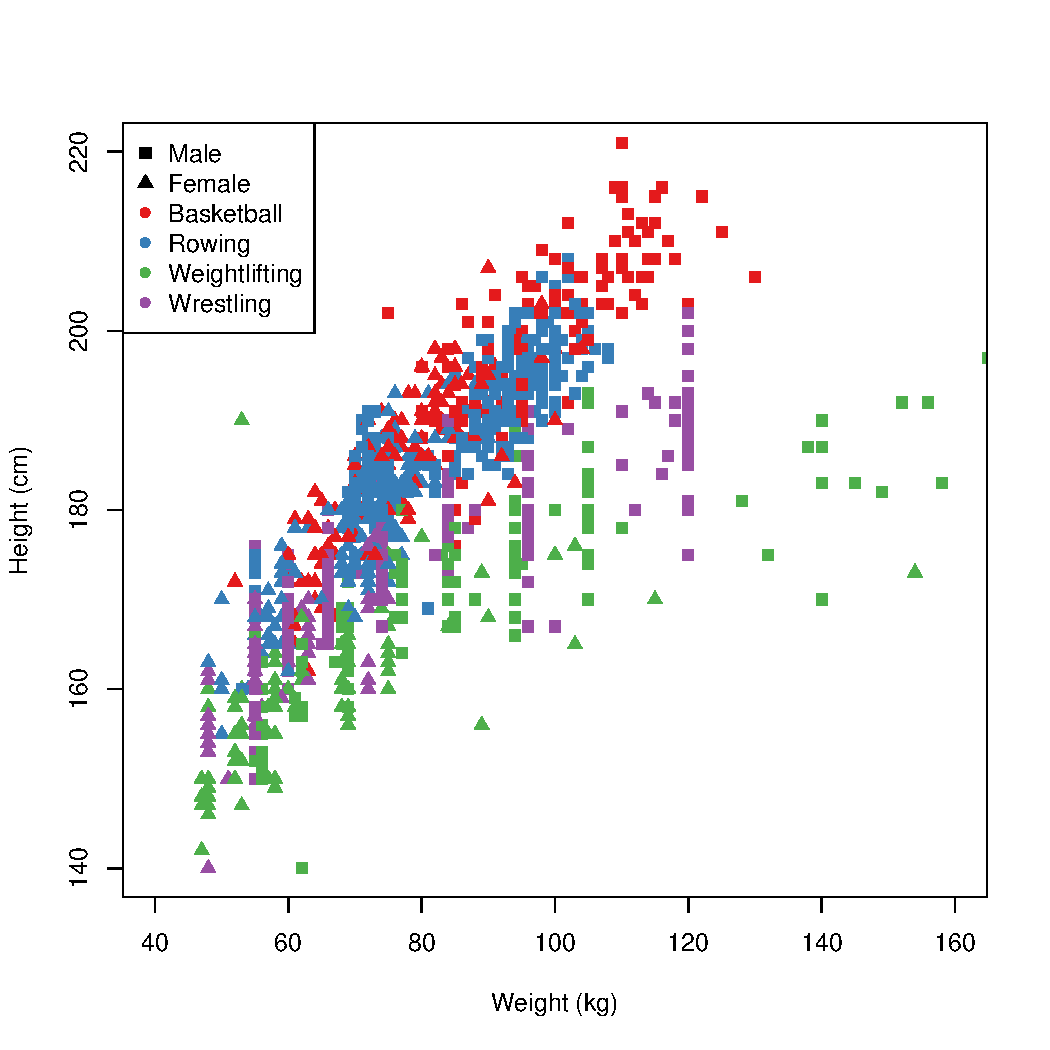
\includegraphics[scale=0.40]{../graphics/basketball.pdf}
      \end{center}
    \end{minipage}
    \hspace{0.05\textwidth}
    \begin{minipage}{0.45\textwidth}
      \begin{center}
        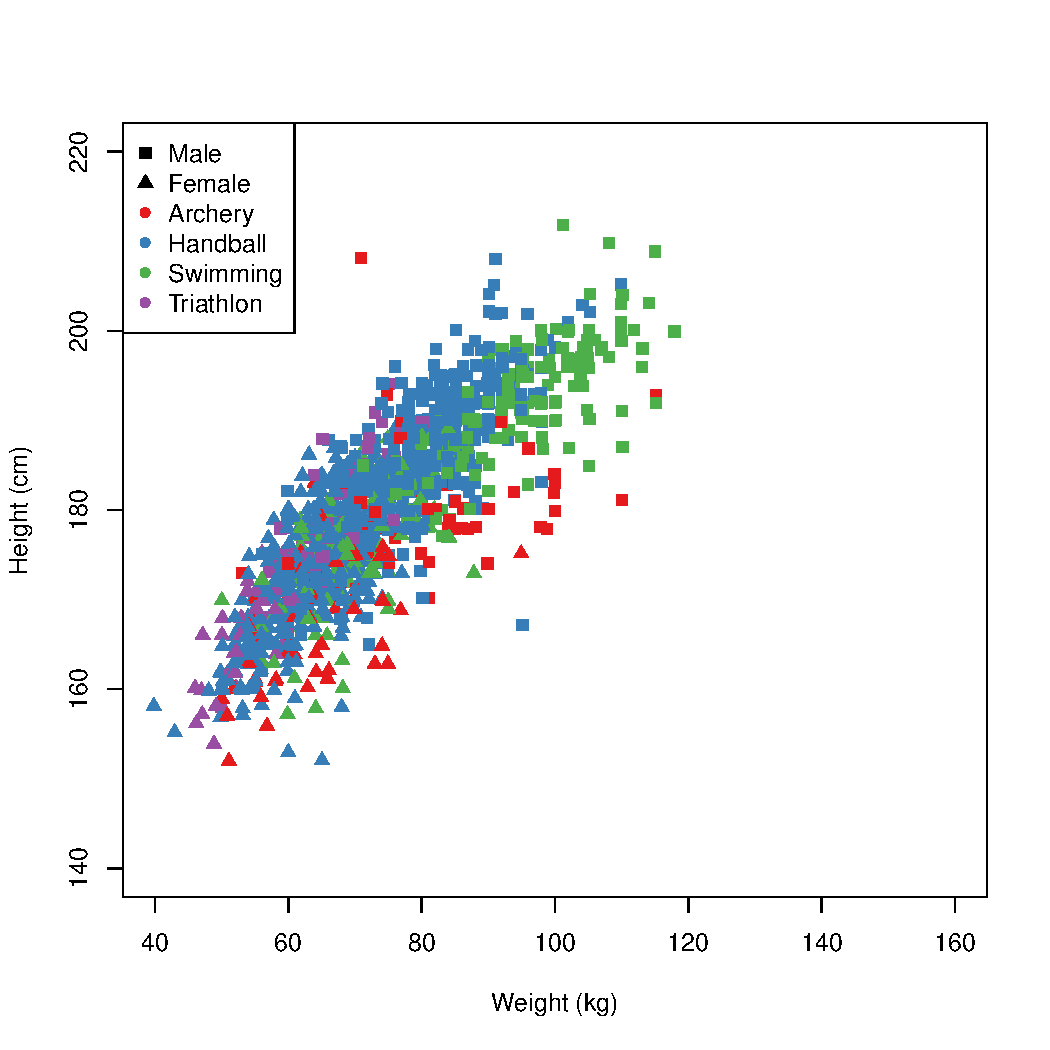
\includegraphics[scale=0.40]{../graphics/swimming.pdf}
      \end{center}
    \end{minipage}
    \caption{Comparing well-differentiated and poorly-differentiated feature clusters for sports classification.}
    \label{sports-features}
   \end{figure} 
\end{center} 

\begin{center}
  \begin{figure}
    \begin{minipage}{0.45\textwidth}
      \begin{center}
        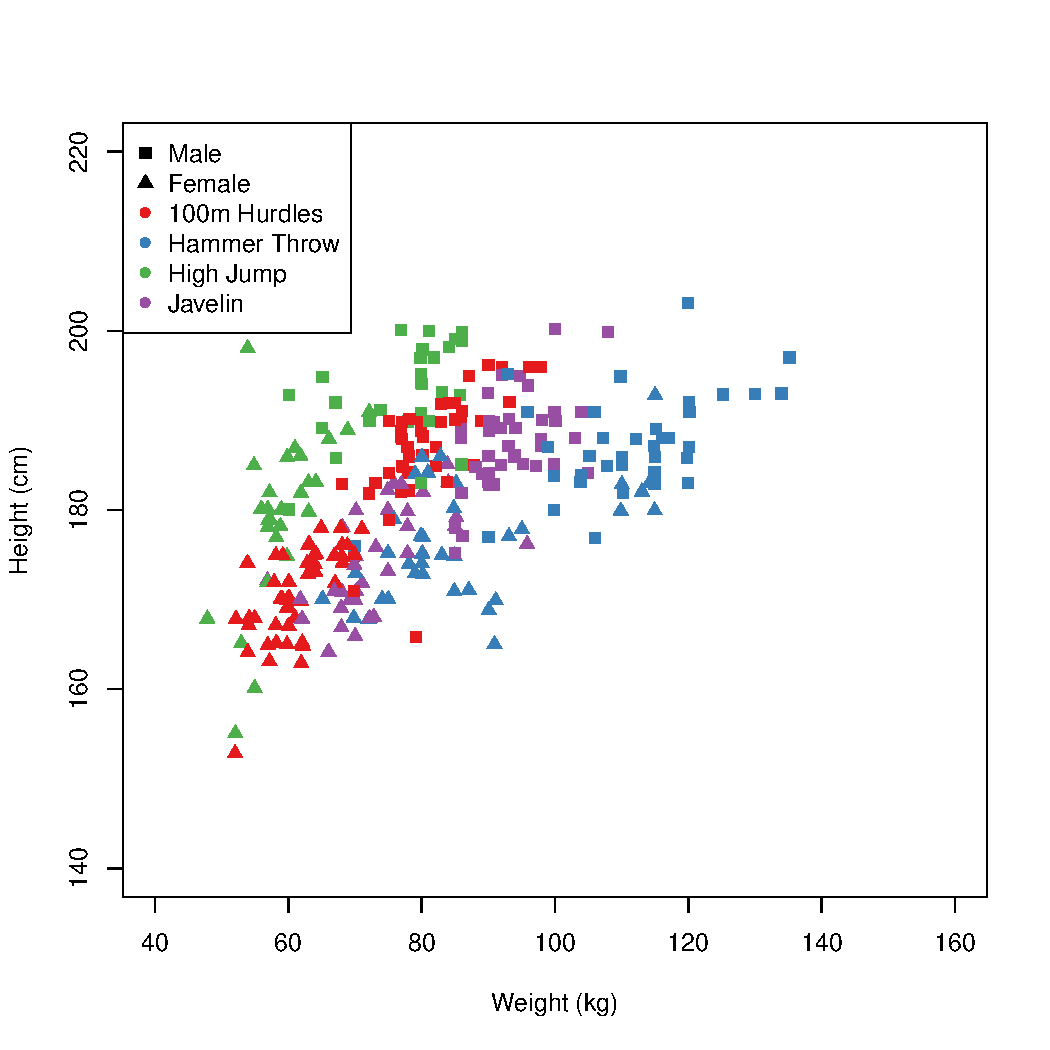
\includegraphics[scale=0.40]{../graphics/javelin.pdf}
      \end{center}
    \end{minipage}
    \hspace{0.05\textwidth}
    \begin{minipage}{0.45\textwidth}
      \begin{center}
        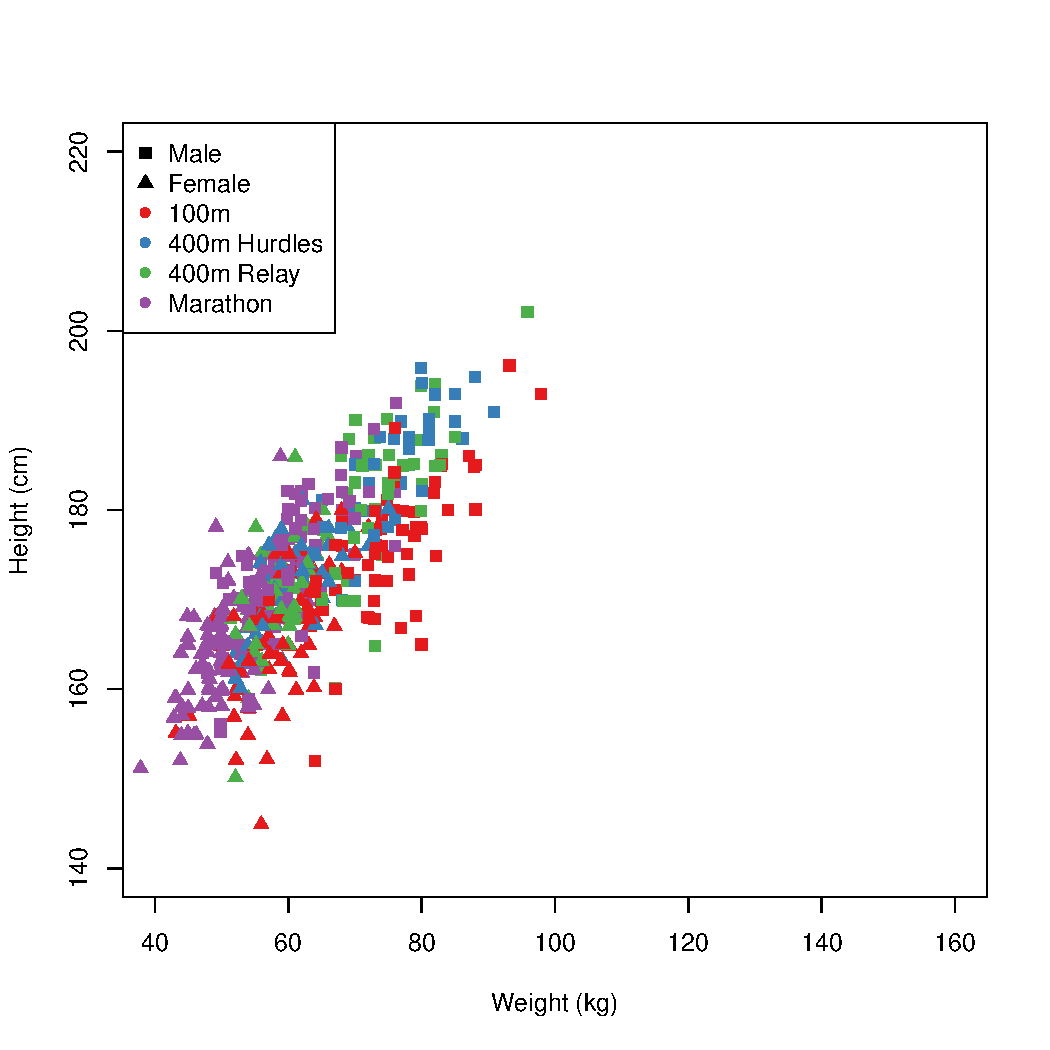
\includegraphics[scale=0.40]{../graphics/marathon.pdf}
      \end{center}
    \end{minipage}
    \caption{Comparing well-differentiated and poorly-differentiated feature clusters for event classification.}
    \label{events-features}
   \end{figure} 
\end{center} 


\subsection{Model}


% Please specify the random variables and parameters in your model (for example, xi ∈ R are real-valued and yj are categorical variables), and 

In order to classify an athlete from the test set, we can use the posterior predictive distribution
\begin{eqnarray*}
p(\mathbf{y}|\mathcal{D}) &=& \sum_{k \in N} w_k p(\mathbf{y}|\mathcal{D}_k),
\end{eqnarray*}
where $w_k$ is the weight on category $k$, $\mathcal{D}_k$ is the feature data for observations in category $k$, and $N$ is the set of categories. Categories can represent sports or events depending on the classification task. The substantive interpretation of the posterior predictive distribution is the probability that a given athlete belongs to a certain category.

% todo: more detail; express generally enough for all 5 models

% provide interpretations for these variables (i.e., which are observed, which are hidden, and which you will be estimating, and how each of the observed values will be processed from the original data). 


\subsection{Machine Learning Methods}

% In three sentences, describe the inference problem and what methods you will use for this task.

Several machine learning methods were used to classify Olympic athletes by sport and event. Hierarchical clustering was performed with a Gaussian likelihood model, with the covariance matrix $\Sigma_k=\lambda_k D_k A D_k^T$ (an ellipsoidal distribution with variable volume, equal shape, and variable orientation) \citep{heller2005bayesian,fraley2012mclust}. Conditional inference trees were formed by recursive binary partitioning, using the \texttt{party} package in $\mathcal{R}$ \citep{hothorn2006unbiased,hothorn2010party}. Evolutionary trees were constructed to be globally optimal by minimizing the misclassification rate, using the \texttt{evtree} package \citep{grubinger2011evtree}. Breiman's Random Forest algorithm was used with 500 trees, as implemented in the \texttt{randomForest} package \citep{liaw2002classification}. Single-hidden-layer neural networks were constructed with 30 units in the hidden layer for sport classification and 50 for event classification, with the package \texttt{nnet} \citep{venables2002modern}.

% In terms of being concise, if the methodological ideas are written exactly elsewhere, you may reference (and cite) that text, as long as you explain clearly what you did so that your experimental results could be replicated based on your text.


\section{Results}

\subsection{Classification by Sport}

Figure \ref{matrices} presents classification matrices for sports (left two columns) and events (right two columns). Each matrix is row-normalized, so the darkest cell on a row indicates the modal predicted class (columns) for true members of the class (rows). Dark cells along the diagonal indicate accurate predictions. A legend is provided in Figure \ref{legend}. Hierarchical clustering was not used for the event classification task (see Section \ref{diagnostics}).

\begin{figure}

  \begin{center}
  % %%%%%%%%%%%%%%%%%%%%%%%%%%%%%%%%%%%%%%%%%%%%%%%%%%%%%%%%
  Hierarchical Clustering \\
  \begin{minipage}{0.20\textwidth}
    % \begin{center}
      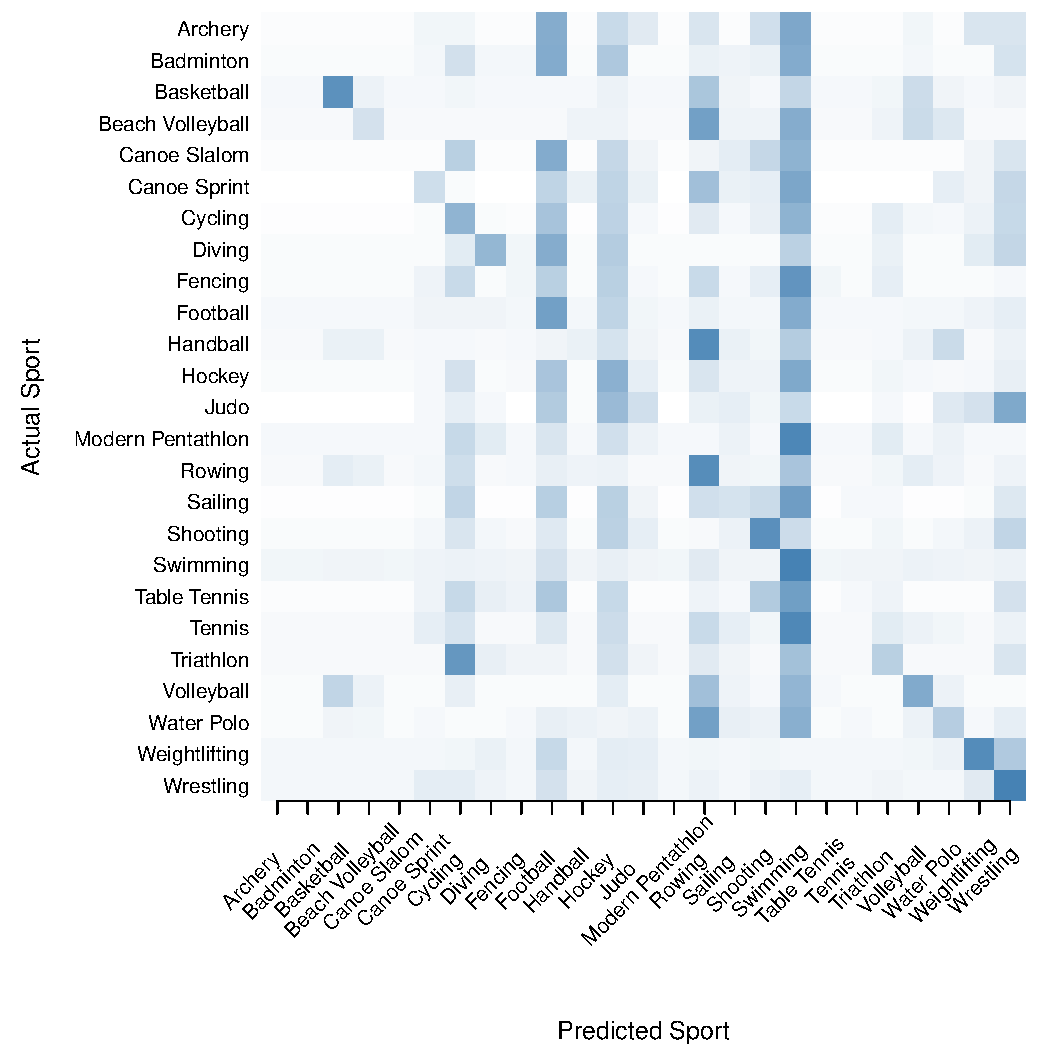
\includegraphics[scale=0.20]{../graphics/sportMclust-trn.pdf}
    % \end{center}
  \end{minipage}
  \hspace{0.05\textwidth}
  \begin{minipage}{0.20\textwidth}
    % \begin{center}
      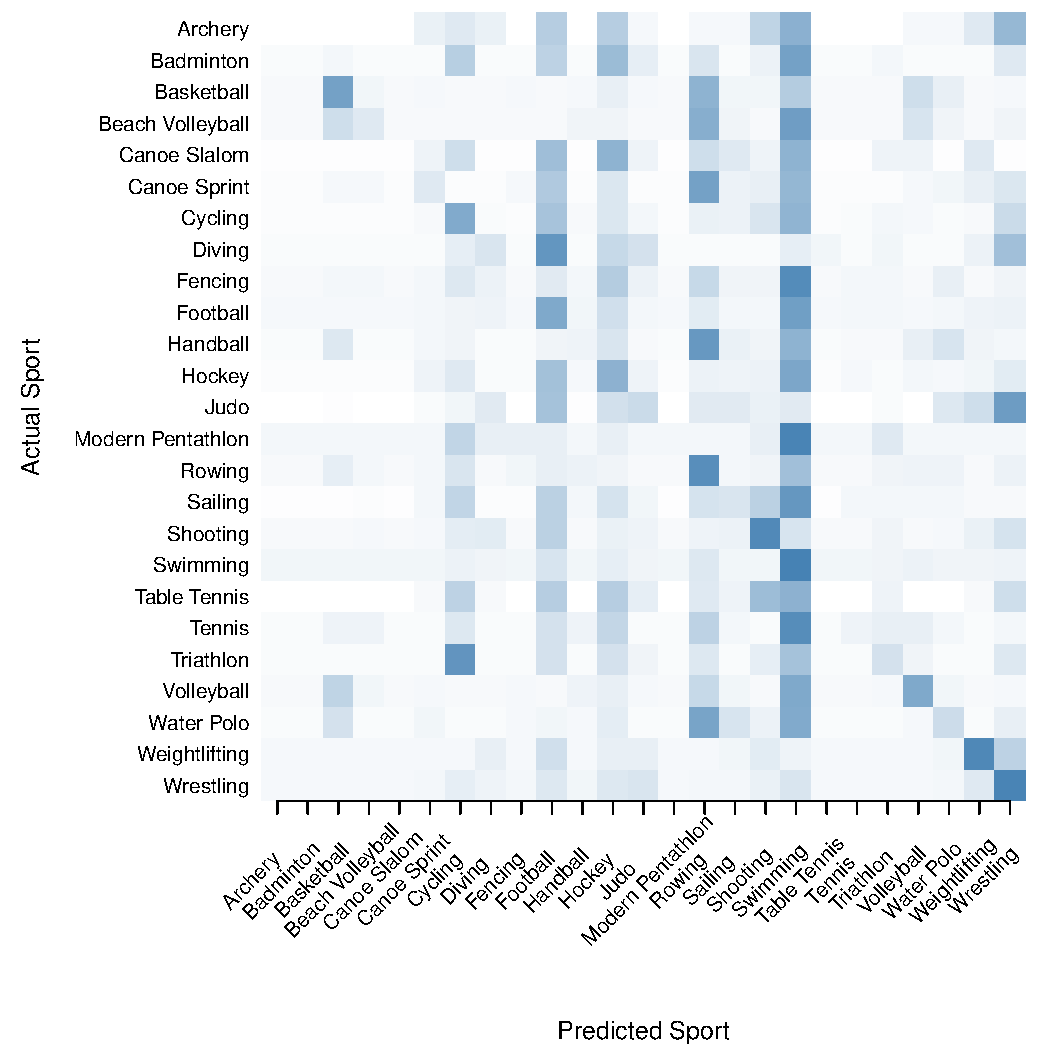
\includegraphics[scale=0.20]{../graphics/sportMclust-tst.pdf}
    % \end{center}
  \end{minipage}


  %%%%%%%%%%%%%%%%%%%%%%%%%%%%%%%%%%%%%%%%%%%%%%%%%%%%%%%%%
    Conditional Inference Tree \\

  \begin{minipage}{0.20\textwidth}
    \begin{center}
      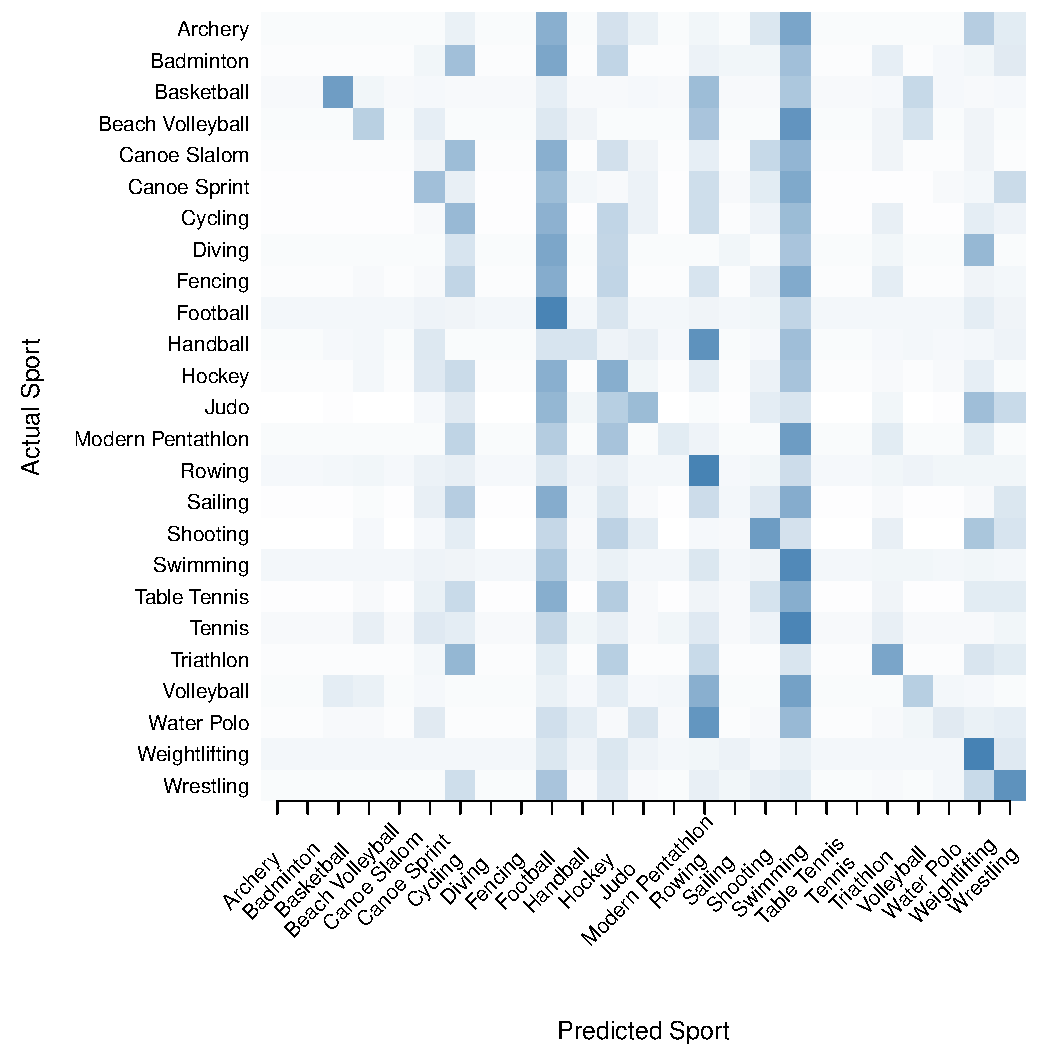
\includegraphics[scale=0.20]{../graphics/sportCIT-trn.pdf}
    \end{center}
  \end{minipage}
  \hspace{0.05\textwidth}
  \begin{minipage}{0.20\textwidth}
    \begin{center}
      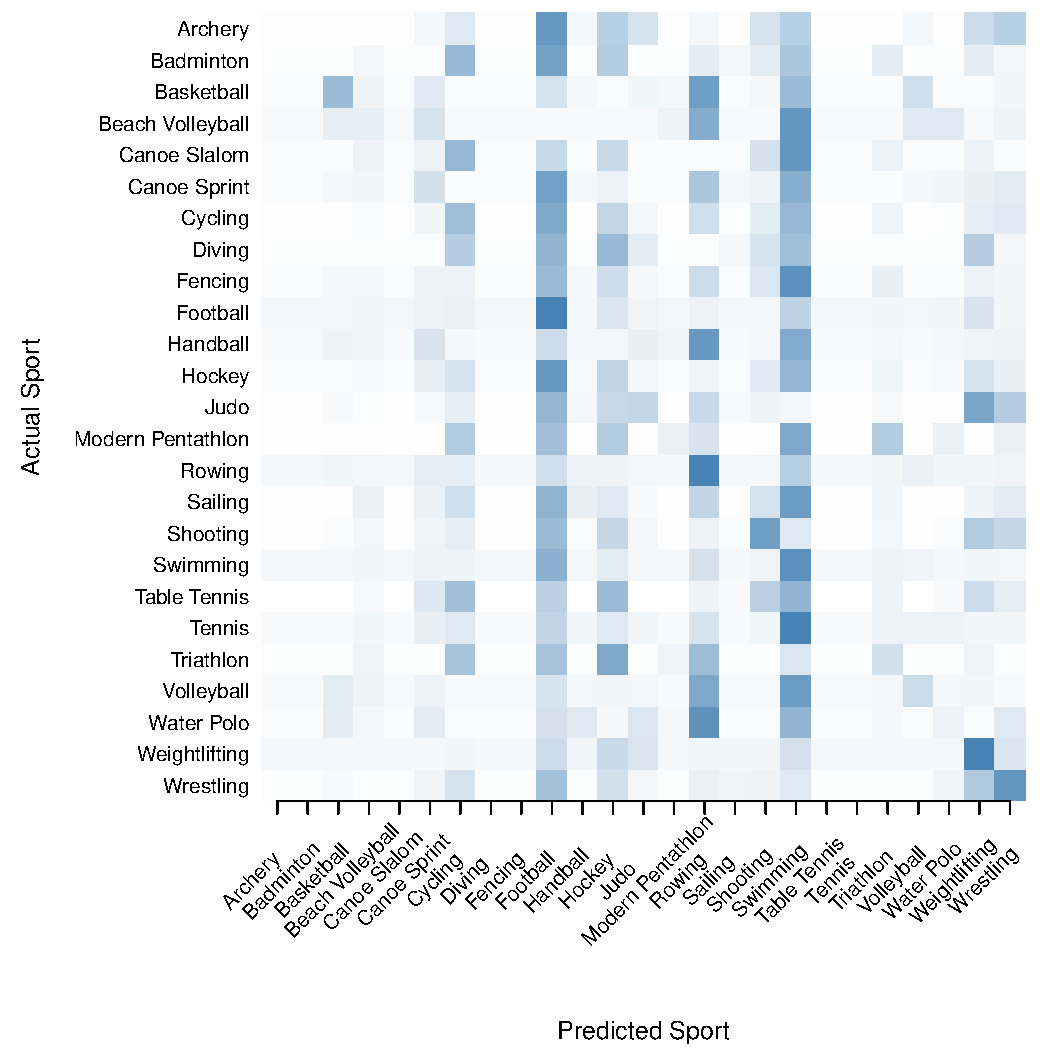
\includegraphics[scale=0.20]{../graphics/sportCIT-tst.pdf}
    \end{center}
  \end{minipage}
  \hspace{0.05\textwidth}
    \begin{minipage}{0.20\textwidth}
    \begin{center}
      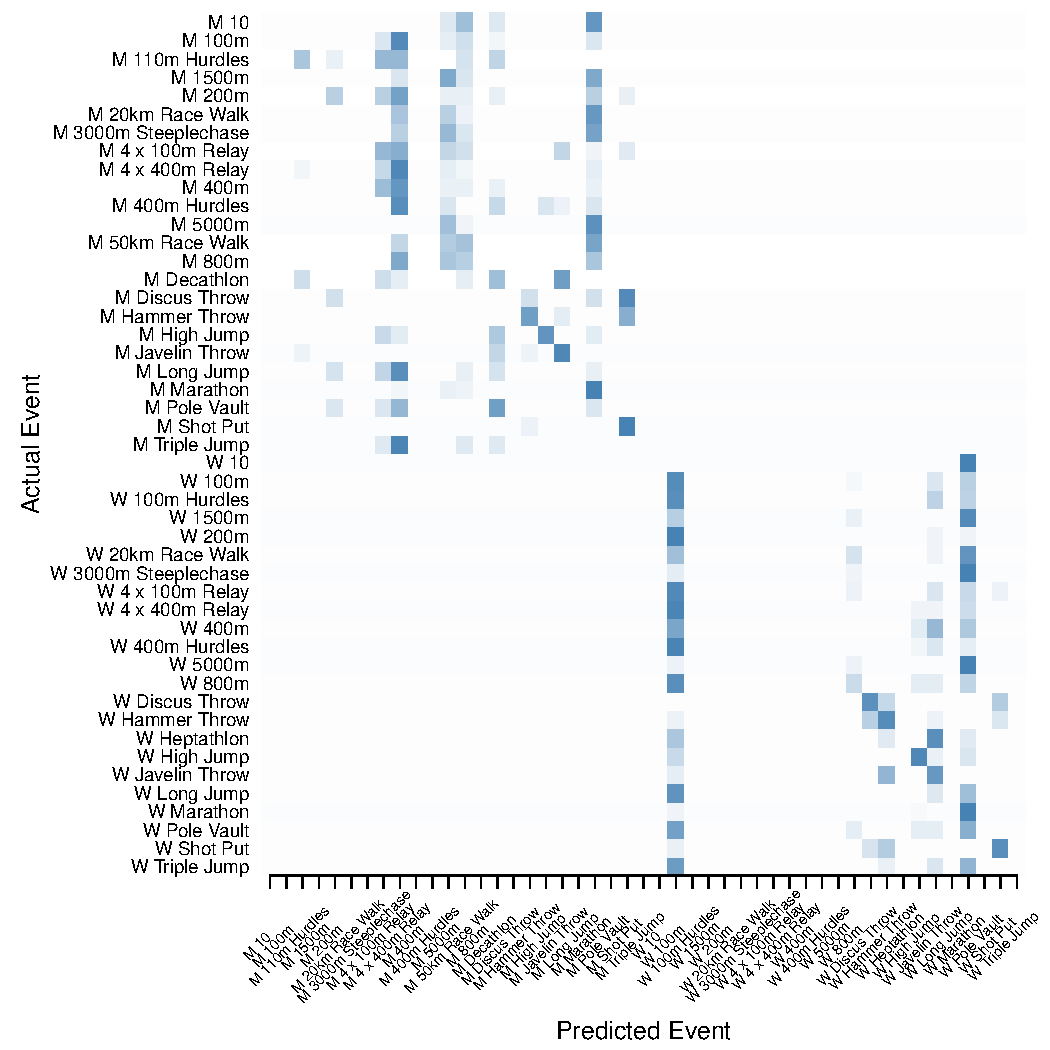
\includegraphics[scale=0.20]{../graphics/athletesCIT-trn.pdf}
    \end{center}
  \end{minipage}
  \hspace{0.05\textwidth}
  \begin{minipage}{0.20\textwidth}
    \begin{center}
      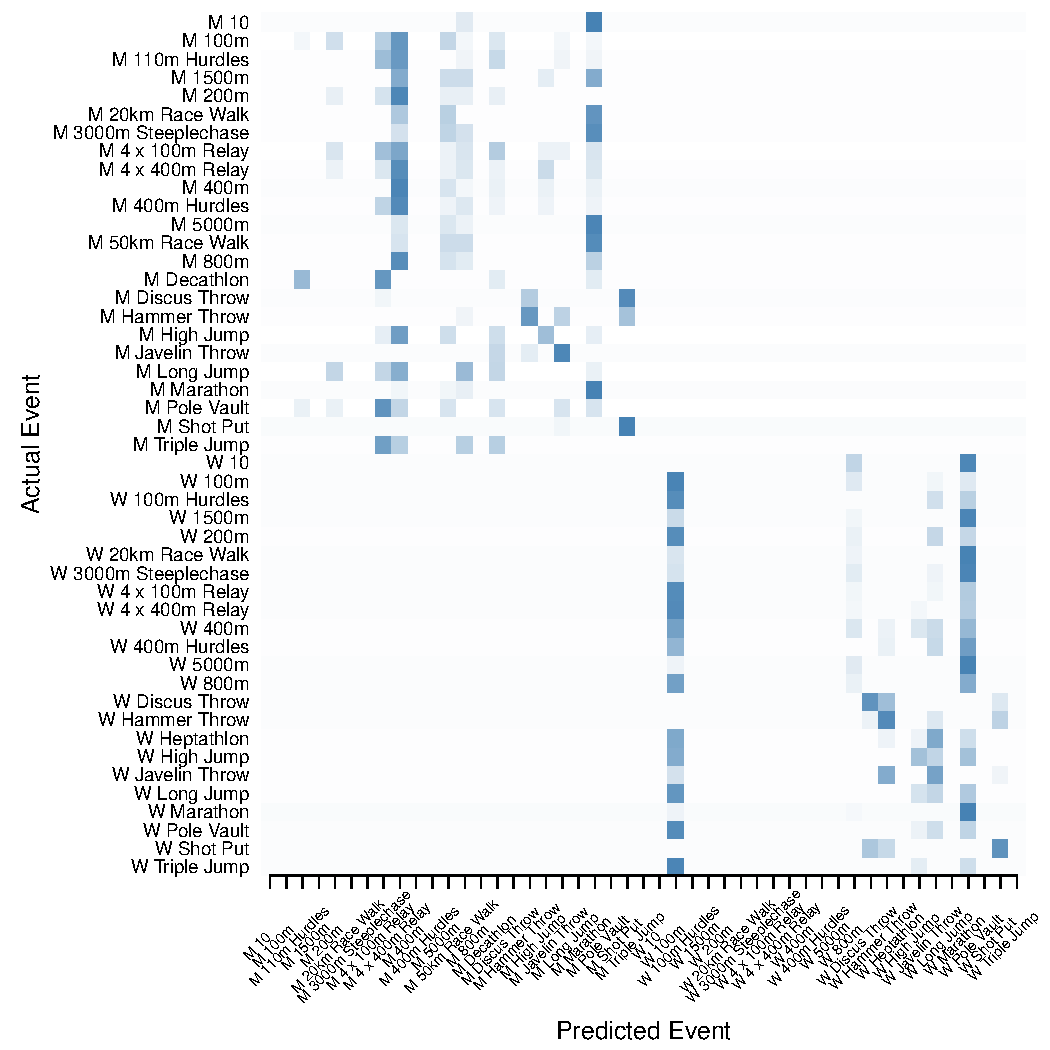
\includegraphics[scale=0.20]{../graphics/athletesCIT-tst.pdf}
    \end{center}
  \end{minipage}



  %%%%%%%%%%%%%%%%%%%%%%%%%%%%%%%%%%%%%%%%%%%%%%%%%%%%%%%%%
    Evolutionary Tree \\

  \begin{minipage}{0.20\textwidth}
    \begin{center}
      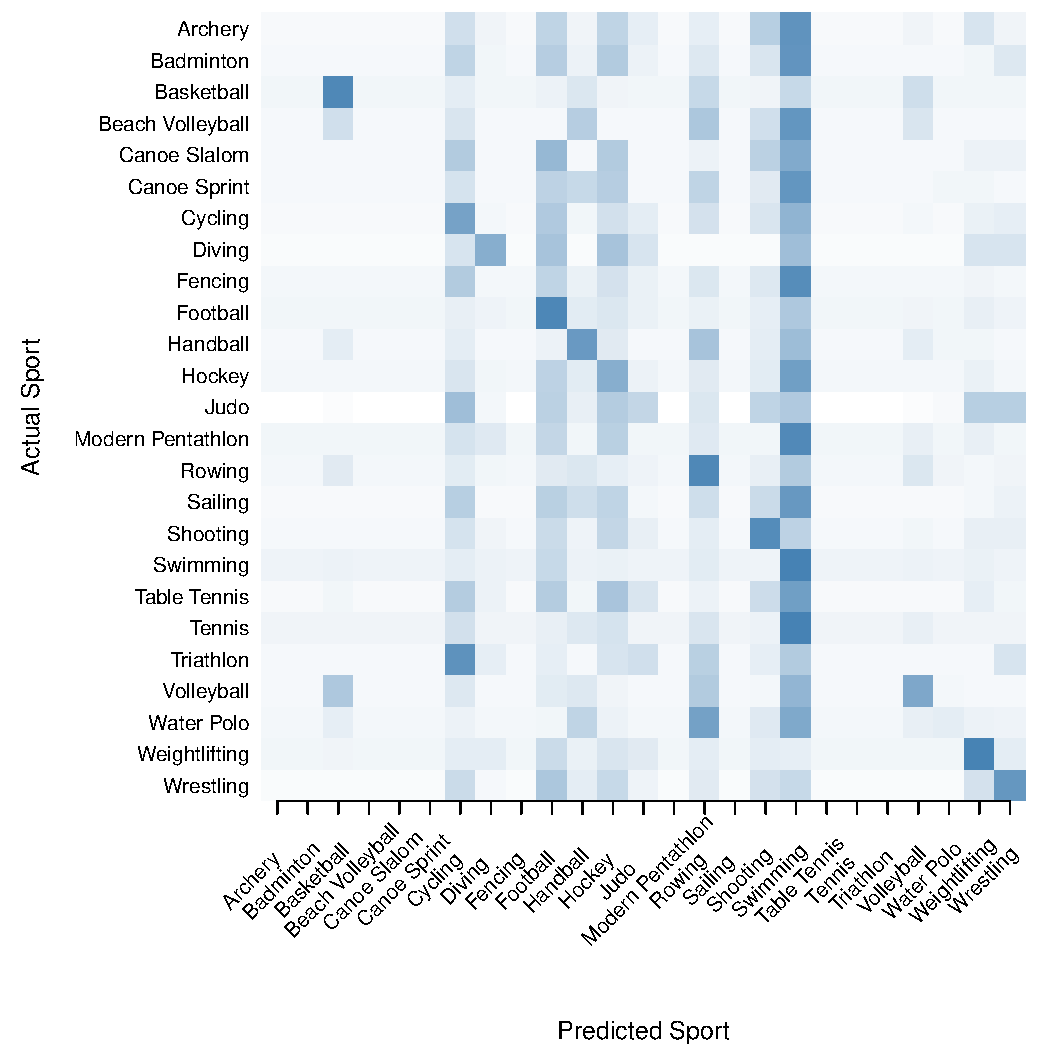
\includegraphics[scale=0.20]{../graphics/sportEV-trn.pdf}
    \end{center}
  \end{minipage}
  \hspace{0.05\textwidth}
  \begin{minipage}{0.20\textwidth}
    \begin{center}
      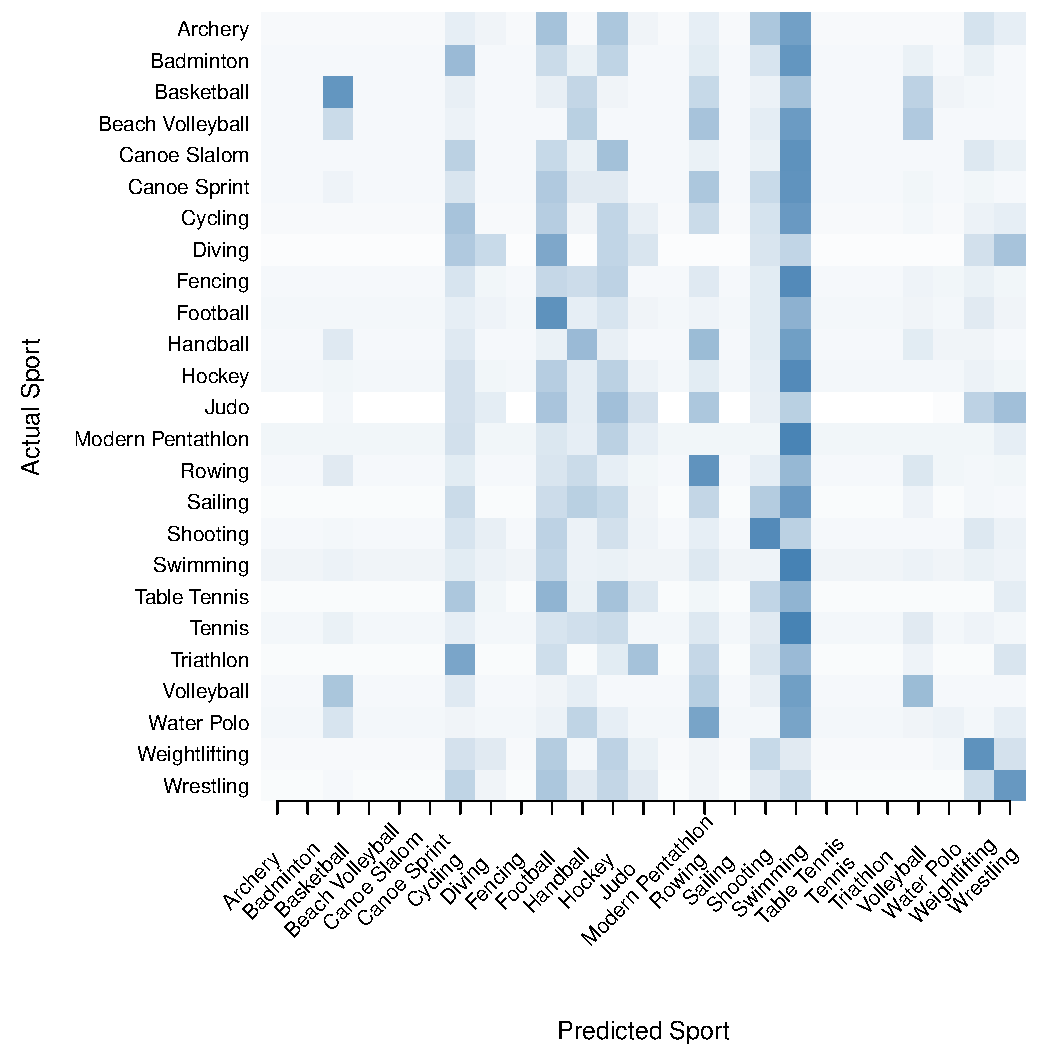
\includegraphics[scale=0.20]{../graphics/sportEV-tst.pdf}
    \end{center}
  \end{minipage}
  \hspace{0.05\textwidth}
    \begin{minipage}{0.20\textwidth}
    \begin{center}
      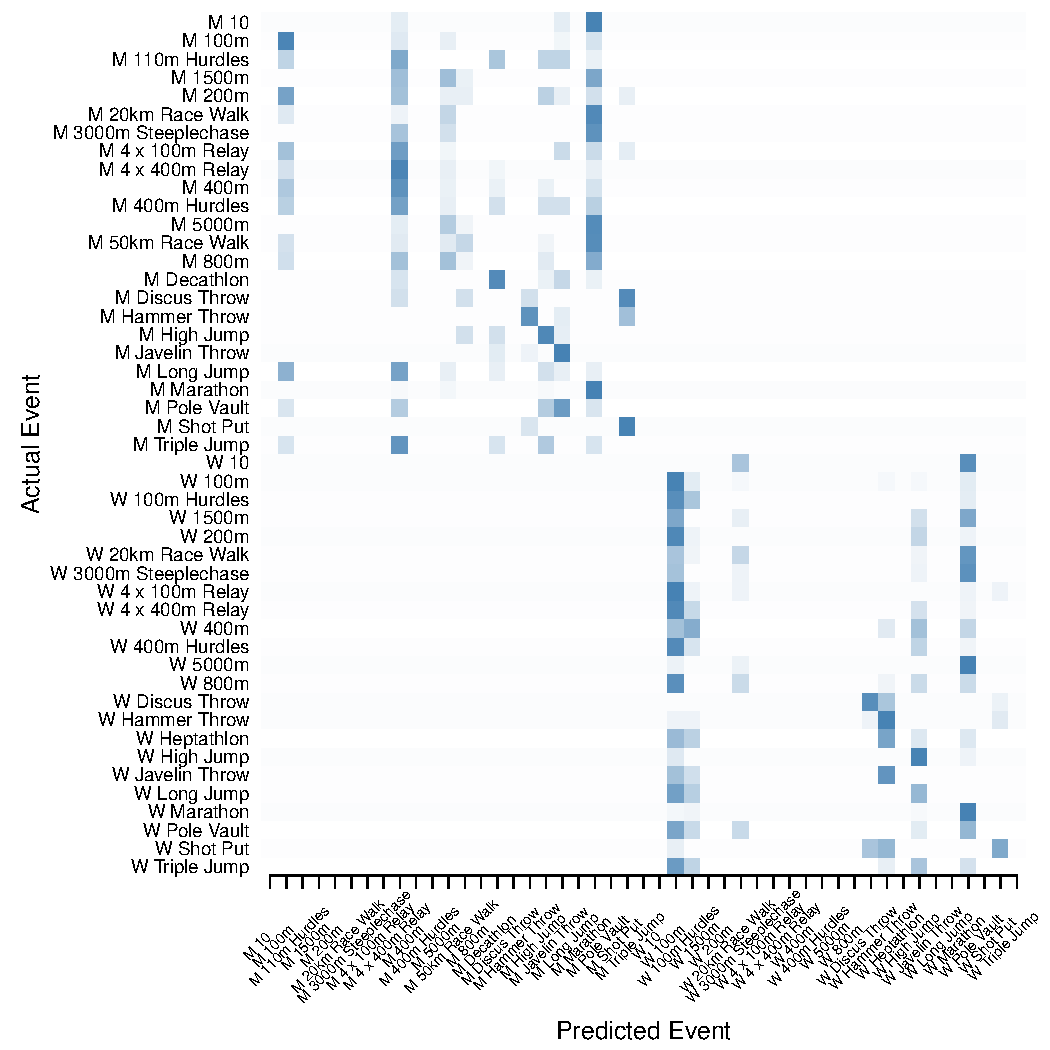
\includegraphics[scale=0.20]{../graphics/athletesEV-trn.pdf}
    \end{center}
  \end{minipage}
  \hspace{0.05\textwidth}
  \begin{minipage}{0.20\textwidth}
    \begin{center}
      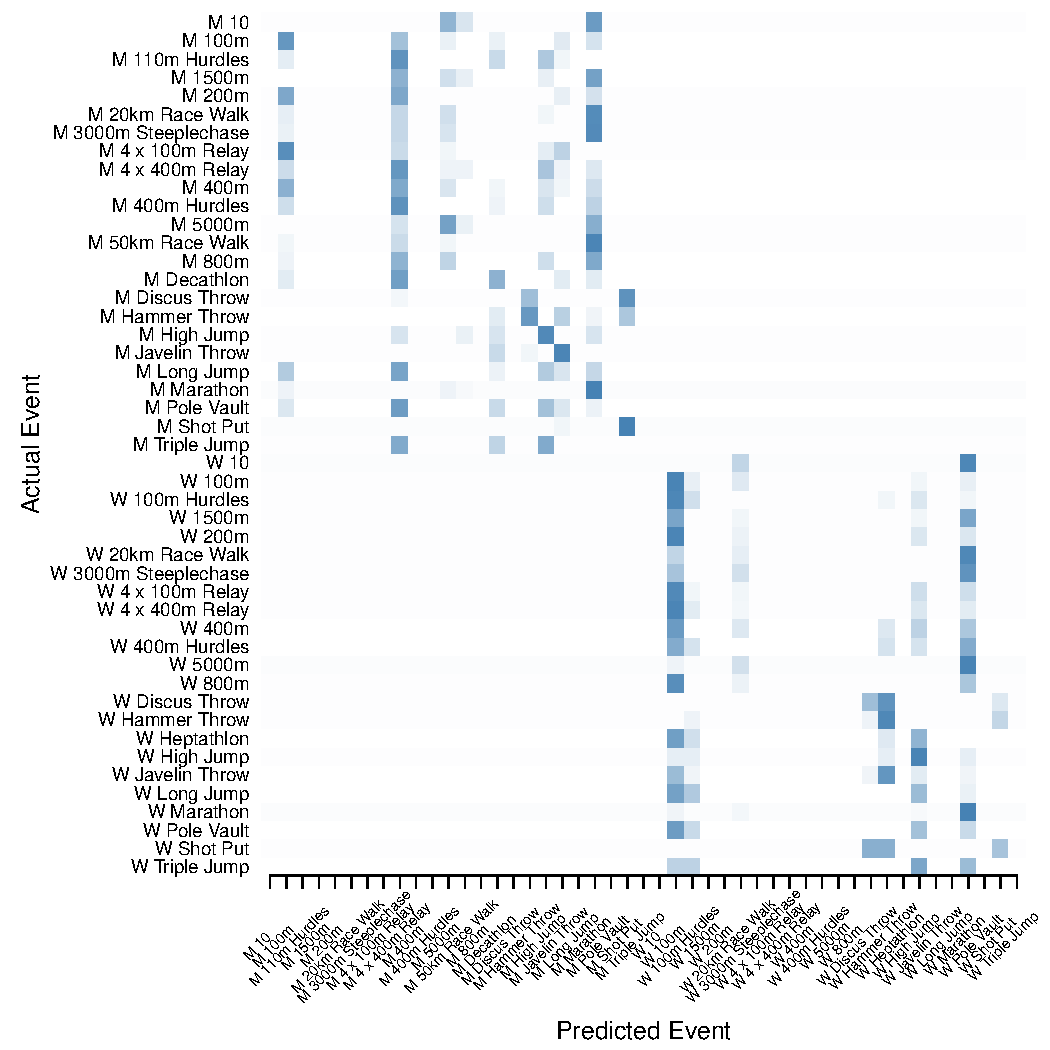
\includegraphics[scale=0.20]{../graphics/athletesEV-tst.pdf}
    \end{center}
  \end{minipage}


  %%%%%%%%%%%%%%%%%%%%%%%%%%%%%%%%%%%%%%%%%%%%%%%%%%%%%%%%%
    Random Forest \\
  \begin{minipage}{0.20\textwidth}
    \begin{center}
      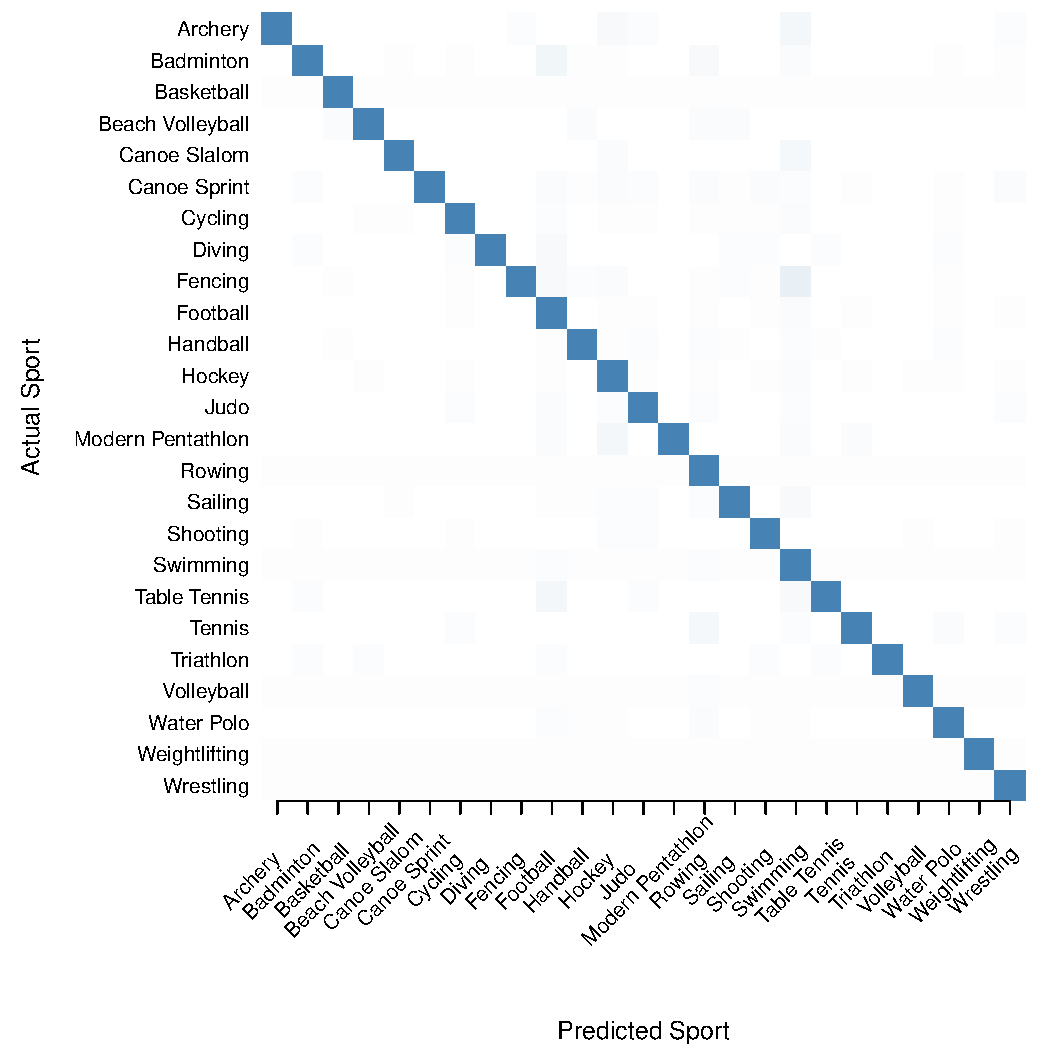
\includegraphics[scale=0.20]{../graphics/sportRF-trn.pdf}
    \end{center}
  \end{minipage}
  \hspace{0.05\textwidth}
  \begin{minipage}{0.20\textwidth}
    \begin{center}
      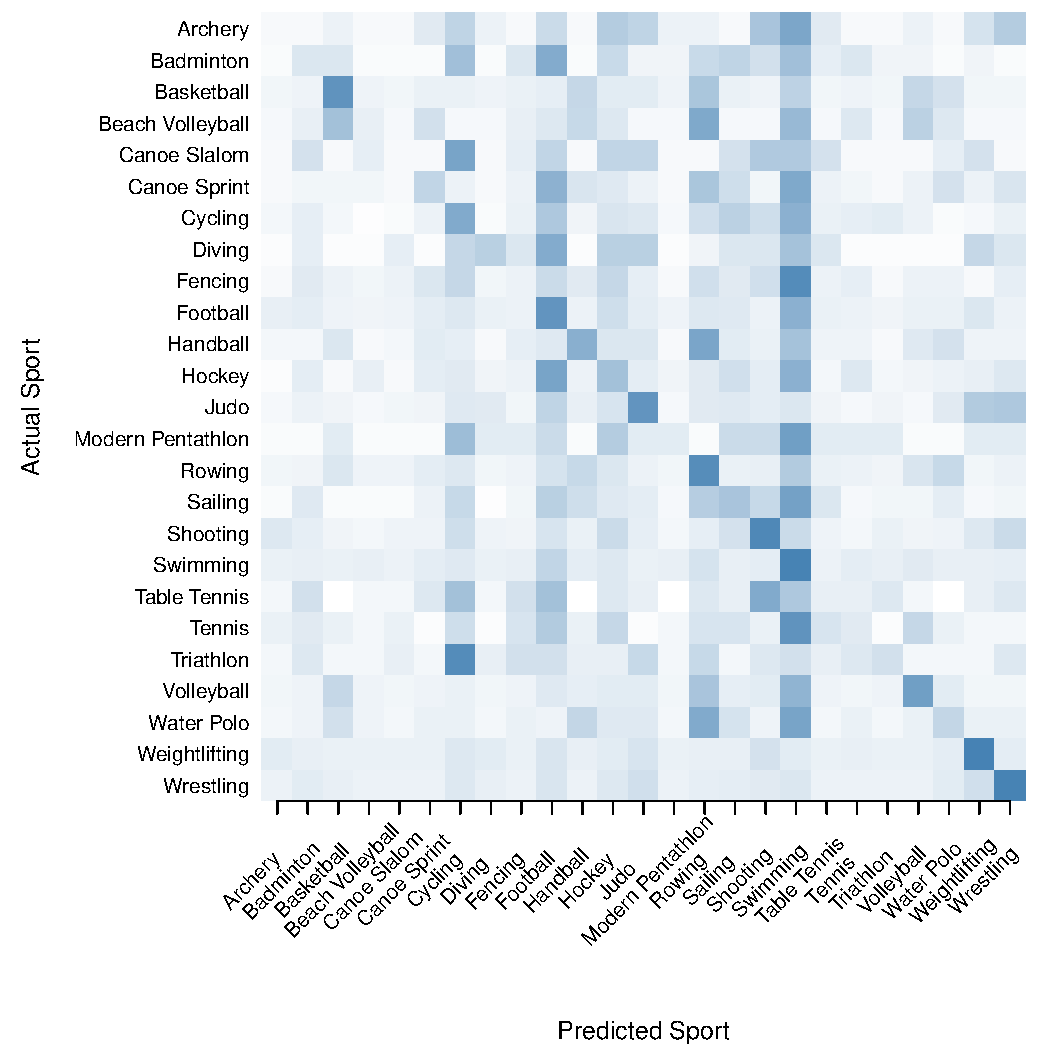
\includegraphics[scale=0.20]{../graphics/sportRF-tst.pdf}
    \end{center}
  \end{minipage}
    \hspace{0.05\textwidth}
    \begin{minipage}{0.20\textwidth}
    \begin{center}
      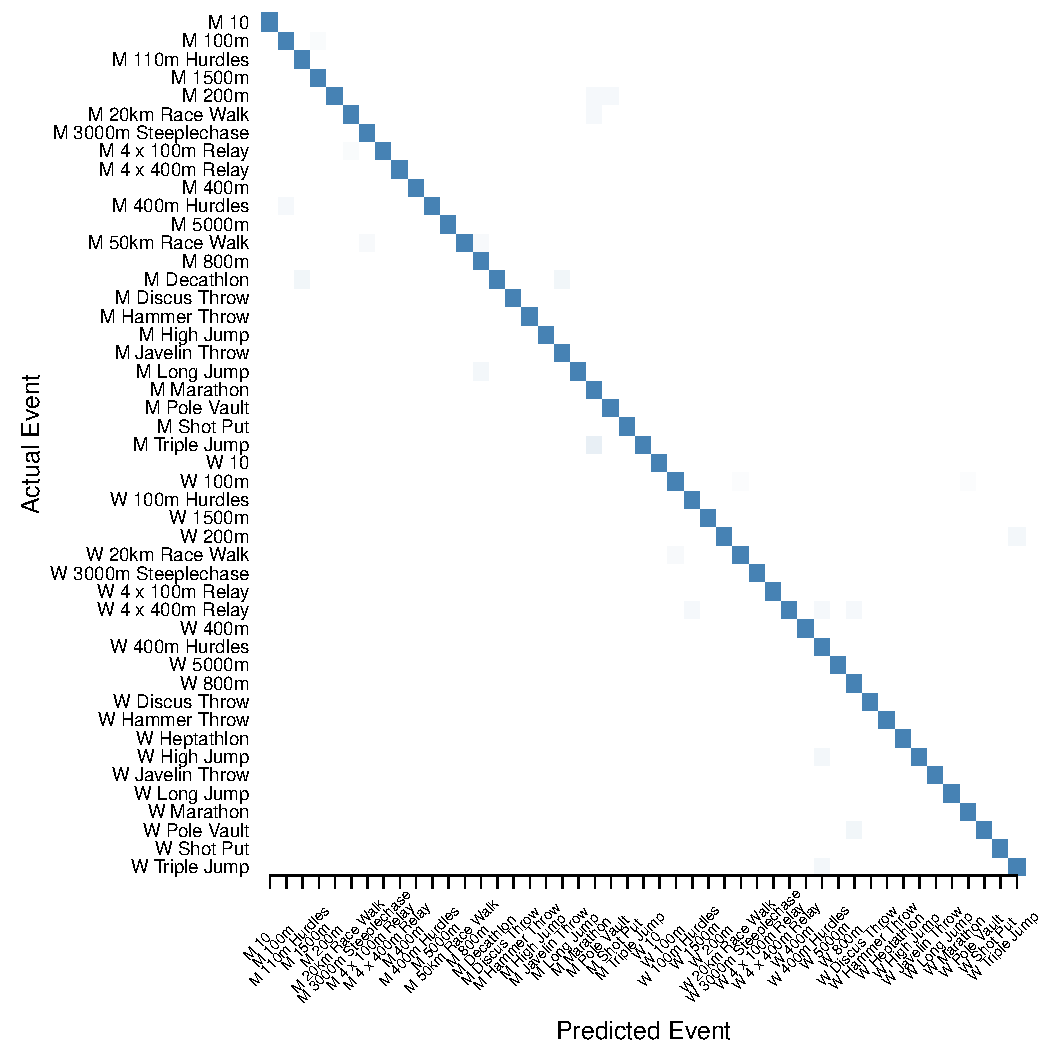
\includegraphics[scale=0.20]{../graphics/athletesRF-trn.pdf}
    \end{center}
  \end{minipage}
  \hspace{0.05\textwidth}
  \begin{minipage}{0.20\textwidth}
    \begin{center}
      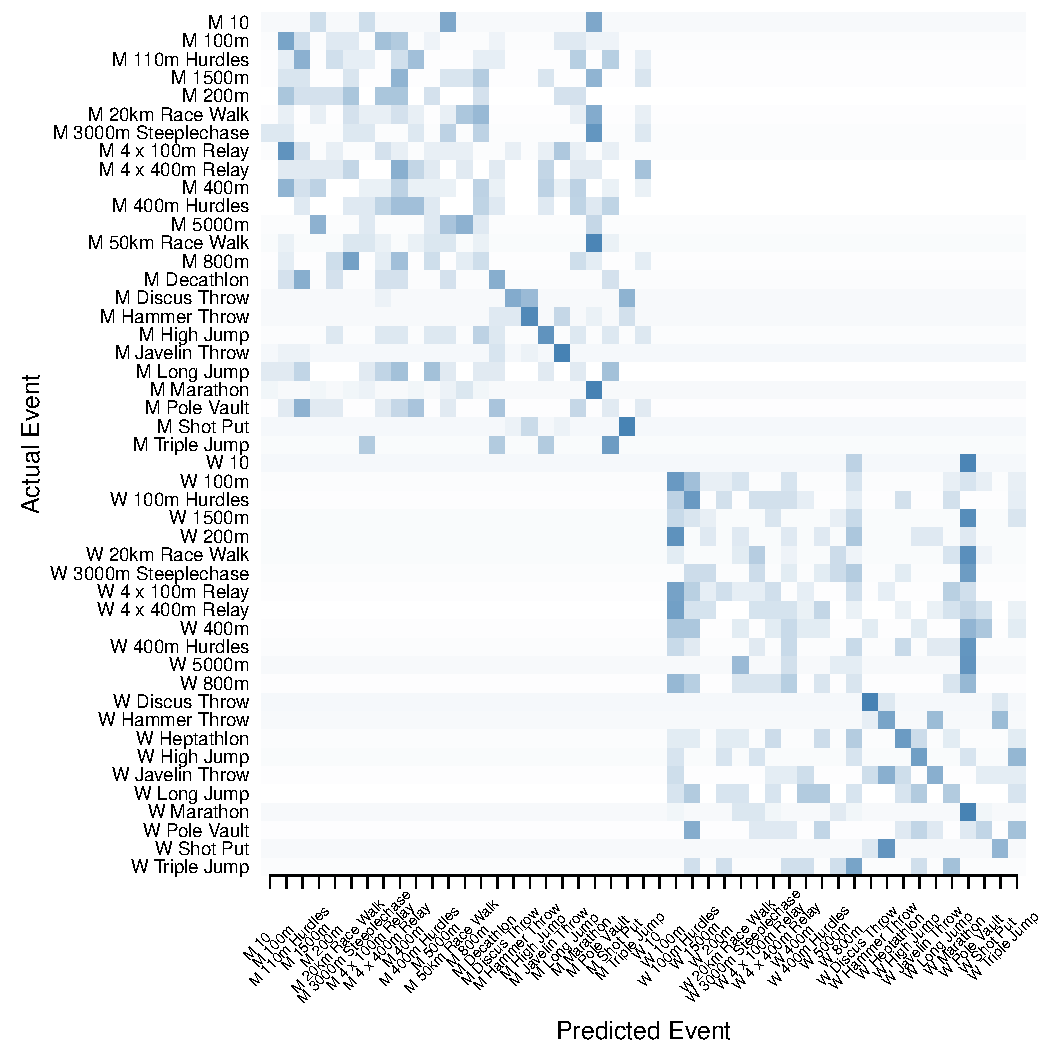
\includegraphics[scale=0.20]{../graphics/athletesRF-tst.pdf}
    \end{center}
  \end{minipage}



  %%%%%%%%%%%%%%%%%%%%%%%%%%%%%%%%%%%%%%%%%%%%%%%%%%%%%%%%%
    Neural Network \\
  \begin{minipage}{0.20\textwidth}
    \begin{center}
      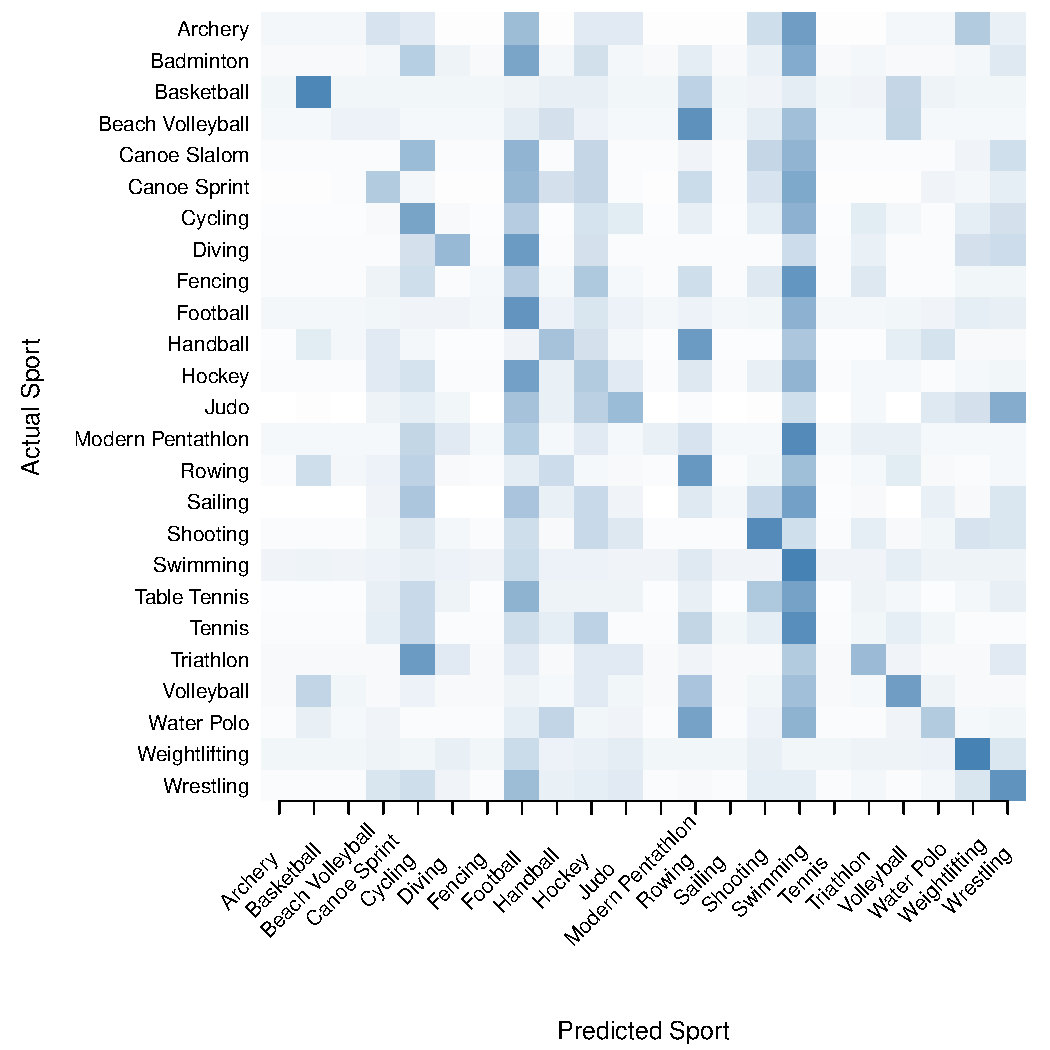
\includegraphics[scale=0.20]{../graphics/sportANN-trn.pdf}
    \end{center}
  \end{minipage}
  \hspace{0.05\textwidth}
  \begin{minipage}{0.20\textwidth}
    \begin{center}
      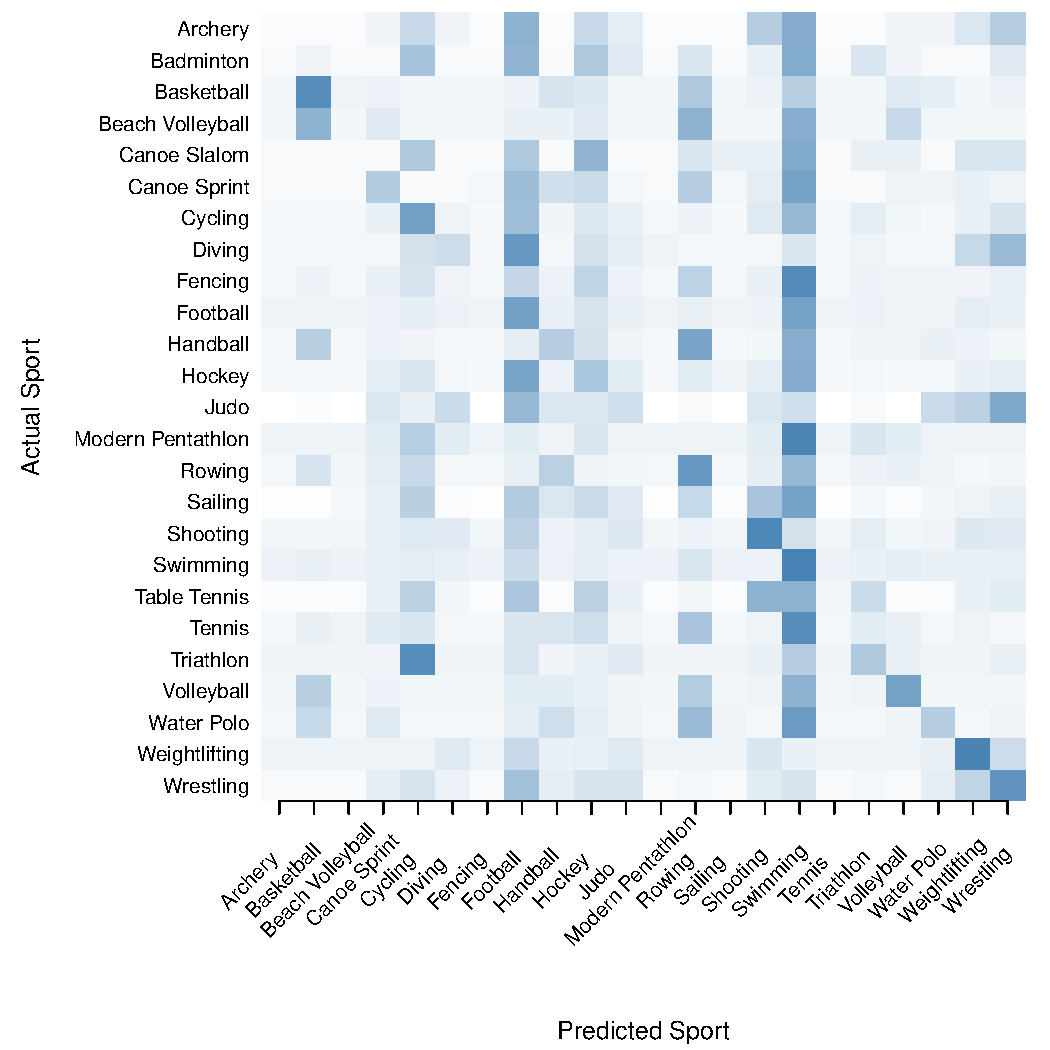
\includegraphics[scale=0.20]{../graphics/sportANN-tst.pdf}
    \end{center}
  \end{minipage}
    \hspace{0.05\textwidth}
    \begin{minipage}{0.20\textwidth}
    \begin{center}
      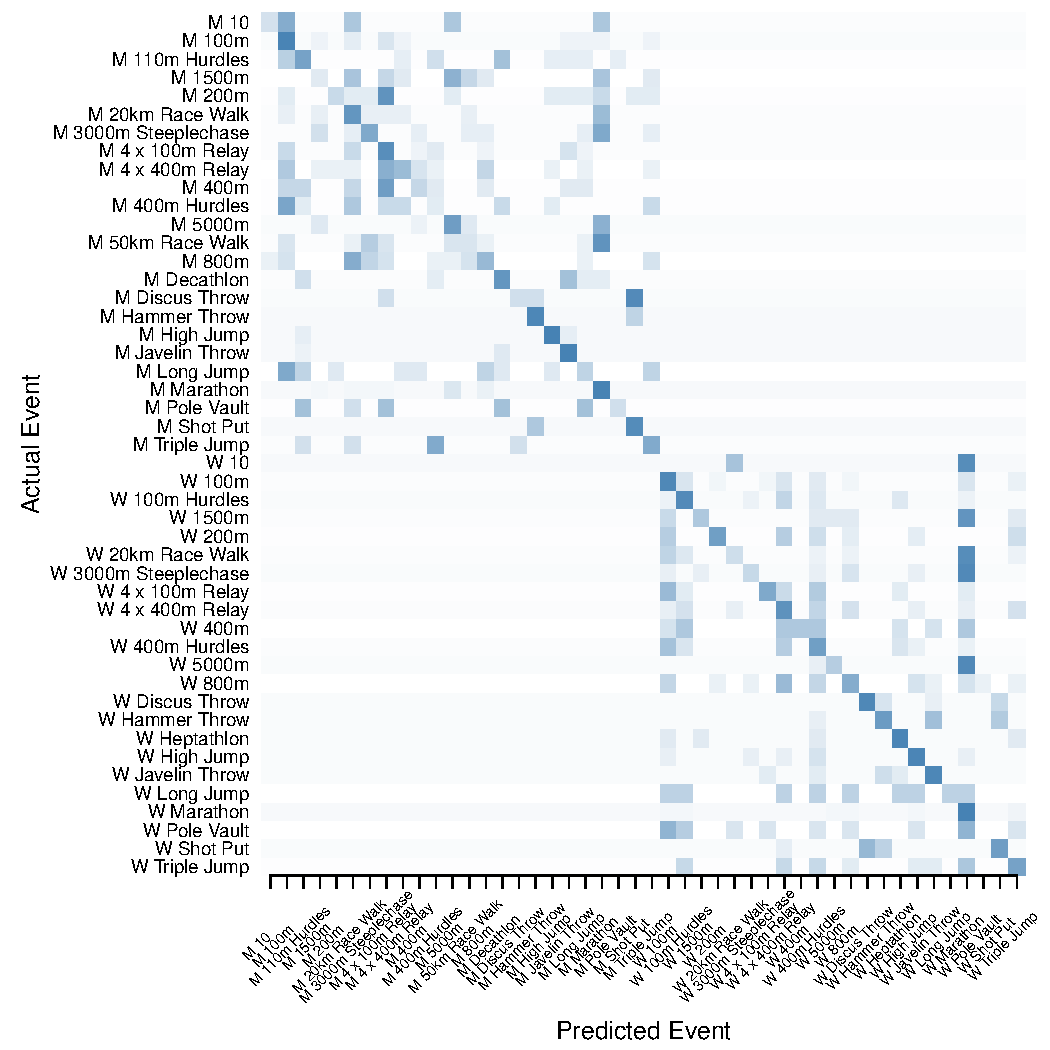
\includegraphics[scale=0.20]{../graphics/athletesANN-trn.pdf}
    \end{center}
  \end{minipage}
  \hspace{0.05\textwidth}
  \begin{minipage}{0.20\textwidth}
    \begin{center}
      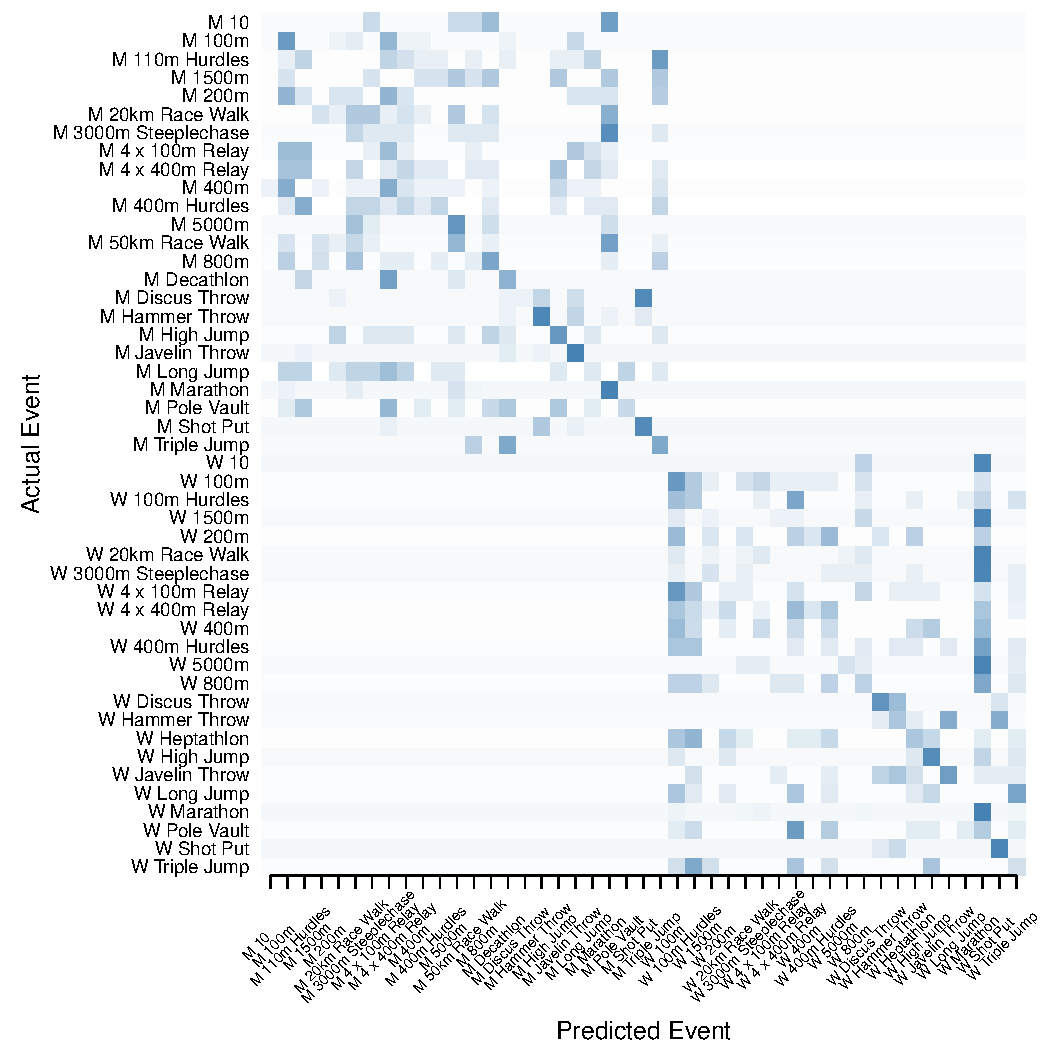
\includegraphics[scale=0.20]{../graphics/athletesANN-tst.pdf}
    \end{center}
  \end{minipage}

  \end{center}

\caption{Classification matrices by method for sports (left two columns) and events (right two columns). Participants' actual sports/events are labeled on the rows of each image, and the predicted sports/events are labeled on the columns. The cells represent row-normalized frequencies. Darker shades on the diagonal indicate accurate classification.}
\label{matrices}
\end{figure}

\begin{figure}
  \begin{center}
    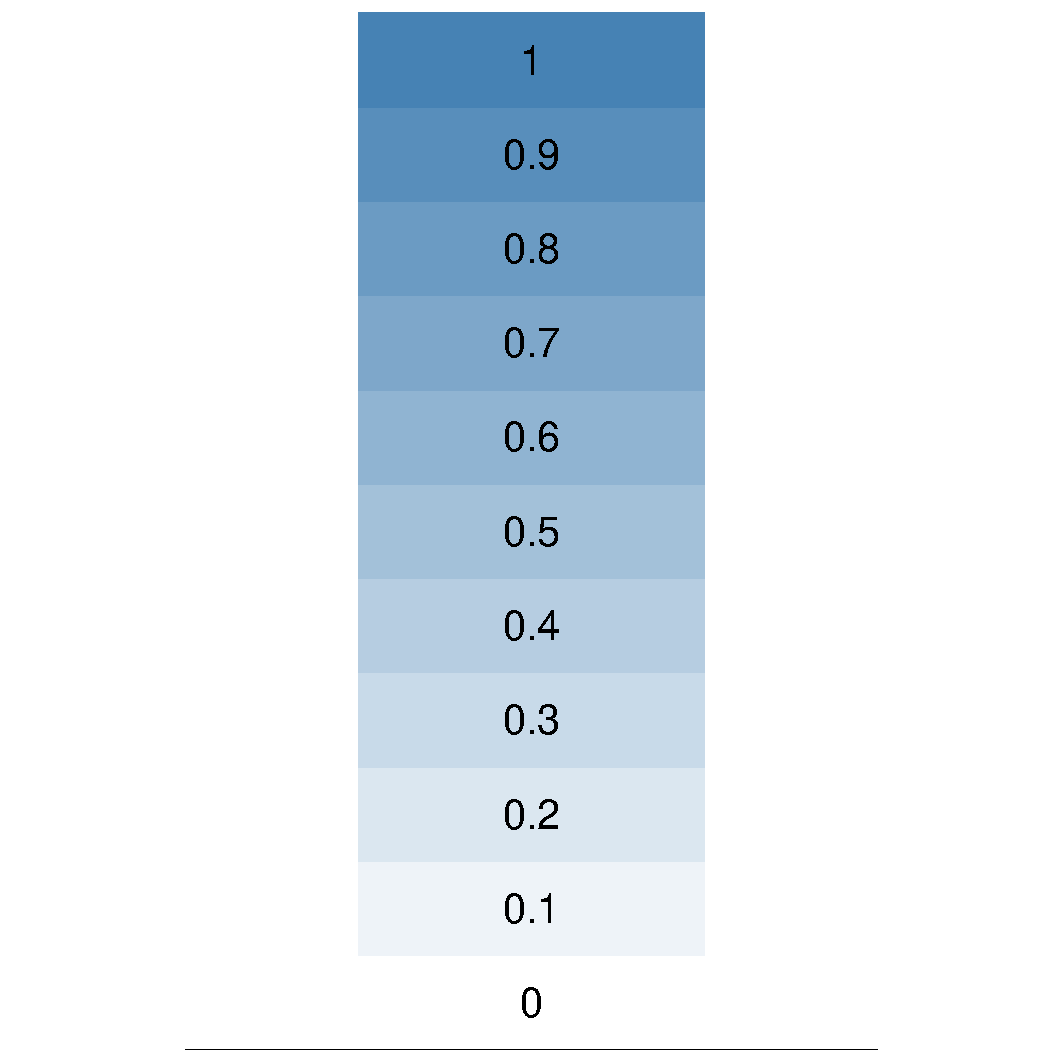
\includegraphics[scale=0.2]{../graphics/scale.pdf}
  \end{center}
  \caption{Legend for matrices in Figure \ref{matrices}.}
  \label{legend}
\end{figure}

\subsection{Model Diagnostics}
\label{diagnostics}

Table \ref{accuracy} presents the accuracy of each model for the sport and event classification tasks. Hierarchical clustering could not be used for event classification due to the small sizes of the clusters (for example, there was complete data for only one participant in the women's triathlon event). The ratio columns indicate how well the model performs on the test data relative to the training data. Values near one mean that the model does about as well out-of-sample as it does on the training data, while values near zero suggests a model that is overfit to the trianing data.

\begin{table}[h!]
\caption{Accuracy for training and test sets.}
\label{accuracy}
\begin{center}
  % \footnotesize
    \begin{tabular}{lcccccc}
      \multicolumn{1}{c}{} & \multicolumn{3}{c}{Sports} & \multicolumn{3}{c}{Events} \\
       \multicolumn{1}{c}{} & \multicolumn{1}{c}{Train} & \multicolumn{1}{c}{Test} & \multicolumn{1}{c}{Ratio} & \multicolumn{1}{c}{Train} & \multicolumn{1}{c}{Test} & \multicolumn{1}{c}{Ratio}\\
      \midrule
      Hierarchical Clustering     & .272 & .271 & .998 \\
      Conditional Inference Tree  & .279 & .219 & .784 & .277 & .218 & .787 \\
      Evolutionary Tree           & .292 & .236 & .807 & .303 & .230 & .757 \\
      Random Forest               & .923 & .244 & .265 & .976 & .228 & .233 \\
      Neural Network              & .280 & .265 & .949 & .397 & .249 & .623
    \end{tabular}
  \end{center}
\end{table}

\subsection{Interpretation}

Hierarchical clustering had the best test set performance, suggesting a robust model that predicts moderately accurately without overfitting the training data. Evolutionary trees and neural networks both exhibit higher accuracy for events than sports, and maintain acceptable out-of-sample accuracy. Conditional inference trees do slightly less well for both training and test sets. Random forests tend to overfit the training data but still do well on the test set. Overall, this appears to be a difficult classification problem.

% Participants in some sports and events are easier to classify than others. For the sports classification task, basketball, rowing, weightlifting, and wrestling tended to be predicted accurately while archery, handball, swimming, and triathlon were among the least accurately predicted categories. When classifying events, 100m hurdles, hammer throw, high jump, and javelin were predicted fairly accurately, while the 100m race, 400m hurdles, 400m relay, and marathon were more difficult to classify.


\section{Conclusion}

The results presented above show that classifying athletes by sport and event can be achieved with moderate accuracy using only a few features. However, Epstein's confidence that he could accurately classify Olympians by only height and weight seems misplaced. Additional features such as arm length and torso length could improve predictive accuracy. Traits of athletes in some sports and events exhibit noticeable clustering, while other categories are less distinct (i.e. multi-modal). Athletes in some sports and events have a well-defined body type, but Olympians exhibit a wide range of physical features. As the Olympics become more competitive, training will continue to play a vital role in sporting success.


\subsubsection*{Acknowledgments}

Thanks to Michael D. Ward and National Science Foundation Grant \#3331808 for support during this project. Any conclusions or errors are the sole responsibility of the author.

% \newpage
\subsubsection*{References}

% CITE A LOT. Any unreferenced methods, prior work, or biological phenomenon, unless it is textbook-common, will be penalized.


\begingroup
\renewcommand{\section}[2]{}
\bibliographystyle{unsrt}
\bibliography{/Users/mcdickenson/Documents/Templates/RefLib.bib}
\endgroup

\end{document}
